\documentclass[preprint,10pt]{sigplanconf}
\usepackage{url}
\usepackage{listings}
\usepackage{subfigure}
\usepackage{times}
\usepackage{multirow}
\usepackage{color}
\usepackage{multicol}
\usepackage{amsmath}
\usepackage{amssymb}
\usepackage{setspace}
\usepackage{graphicx}
\usepackage{xspace}
\usepackage{color}
\usepackage{rotating}

\newcommand{\addtodo}[1]{\textcolor{red}{[To do: #1]}}
\newcommand{\ctrap}{CTrap\xspace}
\newcommand{\ctraps}{CTraps\xspace}
\newcommand{\ctrapsfull}{CTraps-Full\xspace}
\newcommand{\ctrapsmm}{CTraps-NRR\xspace}
\newcommand{\lws}{CTraps-LWS\xspace}
\newcommand{\lwt}{LWT\xspace}


\newcommand{\Caption}[1]{\begin{minipage}{1.0\columnwidth} \caption{#1} \end{minipage}}
\newcommand{\CaptionWide}[1]{\caption{#1}\vspace{-2ex}}
%\doublespacing
\authorinfo{Anonymous for Submission}{}

\title{Efficient Data Provenance Analysis for Concurrent Programs}

%\authorinfo{Brandon Lucia \and Luis Ceze}{University of Washington, Department of Computer Science and Engineering}{\{blucia0a,luisceze\}@cs.washington.edu\\http://sampa.cs.washington.edu\\{\bf In Submission --- Please Do Not Distribute}}

%\author{Anonymous for Submission}
\begin{document}
\maketitle

\begin{abstract}
%Monitoring inter-thread memory dependences in production is useful.  Doing so
%improves debugging information and provides information to dynamic analyses and
%runtime systems.  Prior work that continuously monitors cross-thread
%dependences typically has overheads too high for production.  
We propose {\em last writer slices}, an analysis for shared-memory
multi-threaded programs that tracks {\em data provenance information} in
production code.  Last writer slices dynamically record the thread and
operation that last wrote each variable, reflecting the {\em provenance} of
values.  Provenance helps understand bugs and we provide last writer slices to
programmers during debugging.  We build {\em communication traps}
(\ctraps) using last writer slices.  \ctraps efficiently
monitors and can interpose on operations that share data between
threads.  \ctraps is extensible, exposing inter-thread dependences
to {\em \ctraps applications} that implement arbitrary analyses.  

We implement last writer slicing and \ctraps.  We conduct debugging studies of
real, buggy programs showing last writer slices are useful for debugging.  We
show \ctraps is useful by implementing two concurrency analyses from prior
work.  We evaluate the performance of our designs using server programs
and standard benchmarks.  We show that collecting last writer slices
has low run time overheads (0--15\%) for many applications,including  
memcached, LevelDB, MySQL, and Apache.  We show that \ctraps imposes low 
overheads by default and that overheads scale with analysis complexity.

\end{abstract}

\section{Introduction}
Multi-threaded programming is challenging.  In contrast to sequential
reasoning, multi-threaded programs require complex reasoning about many threads
of control and their interactions.  In shared memory programs, threads interact
by reading and writing memory locations.  Threads' reads and writes interleave
arbitrarily and nondeterministically. Each interleaving can lead to different
behaviors and memory states, some of which may be undesirable, like crashes or
data corruption.  Moreover, because complete concurrency testing is infeasiable
in general, undesirable interleavings can evade testing and lead to production
failures.

The problem we are addressing in this work is that debugging support for
understanding thread interactions is inadequate.  Today, programmers use a
debugger to examine memory contents either during a debugging execution or by
loading a core dump from a failed execution.  Examining the contents of memory
reveals {\em what} the state of the program is ({\em e.g.}, the values of
variables).  Unfortunately, the real question programmers must answer is {\em
why} the state of the program is what it is.  Understanding why a program
entered an undesirable state ({\em e.g.}, crashed) is the key to changing the
code to prevent future executions from entering that state.  Multi-threading
makes this understanding elusive because implicating particular operations in
particular threads for a failure is a complex task.  Aiding developers in this
understanding for failed production executions is important because
hard-to-find bugs may manifest in production only.


%A common approach to this challenge is to reason about dependent memory
%operations.  Memory operations are dependent if their order determines the
%values they read or write.  The utility of dependence information is made
%especially clear by its prevalent use during manual program debugging and in
%support of program analysis tools.

Our approach to solving that problem is to provide the programmer with {\em
provenance} information that can be examined alongside the program's memory
state ({\em i.e.}, core dump).  A value's provenance describes why a memory
location contains its value.  In this work we develop a new provenance tracking
mechanism called {\em last writer slicing} that satisfies these goals.  A
memory location's last writer slice is a record containing the program point
and the identifier of the thread that last wrote data to that memory location.
As the program executes in production, we collect last writer slices for each
potentially shared memory location and those last writer slices record the
provenance of the values stored in those locations.  Last writer slices are
saved with a core dump when the program fails and are available in the debugger
({\em e.g.}, for breakpoint debugging).

We have three goals for last writer slicing:  (1) To collect a general form of
provenance information, not limited to certain values or locations only. (2) To
provide provenance information focused on how threads interact to aid in
understanding concurrency bugs. (3) To engineer our system to have overheads
low enough for use in production, aiming for a 10 -- 50\% maximum overhead. 



%During debugging provenance helps a programmer better understand not just where failures occur, but where values came from, connectng disparate
%parts of a program that interact, leading to a failure.

%In
%summary, the challenges in using provenance to debug concurrent programs are:
%(1) collecting the right information to characterize the concurrent execution
%behavior; and (2) making it efficient enough for general programs running in
%production settings. 

Last writer slices are primarily useful for concurrency debugging, but we 
observe that provenance information is a
useful foundation for implementing other concurrent program analyses.  Several
tools from prior work have used {\em ad hoc} last-writer information as part of
more heavy-weight analyses in domains like bug detection ({\em e.g.},
~\cite{dmtracker,avio}), automatic debugging ({\em e.g.},
~\cite{recon,conseq,cci}), profiling ({\em
e.g.},~\cite{threadclustering, schedpredictionmodel}), and program
understanding~\cite{oshatr}. 

Motivated by these prior {\em ad hoc} efforts, we build a general mechanism
called {\em Communication Traps} or {\em \ctraps} on top of last writer slices
(Section~\ref{sec:ctraps}). \ctraps is useful for implementing dynamic
concurrency analyses, like the ones discussed above.  \ctraps runs alongside a
program and uses last writer slices to identify memory accesses that lead to
{\em communication} between the threads. Communcation occurs when a thread
accesses memory last written by a different thread and \ctraps delivers a {\em
trap} to a thread when it communicates with another thread, giving it
information about how communication occurred.  Programmer-defined {\em trap
handlers} can implement arbitrary analysis using that information. By default,
\ctraps has low overheads that are appropriate production in many cases.  As we
show in our evaluation, the overhead of \ctraps applications scales with the
complexity of their analysis.



%Provenance is also useful in implementing concurrent program analyses.
%Dependence information is also an important part of many program analysis
%tools.    Bug detection~\cite{avio,fasttrack,raceslicing,dmtracker} and
%debugging~\cite{tipslicingsurvey,bugaboo,recon,cci,defuse,conseq,falcon} tools
%analyze inter-thread dependences to find buggy behavior and help programmers
%understand their errors.
%Profilers~\cite{threadclustering,schedpredictionmodel} analyze inter-thread
%dependences to find optimization opportunities.  Dependences are also essential
%to some program understanding systems~\cite{oshatr} and dynamic checkers for
%thread interaction properties~\cite{oshajava,velodrome}.
%Record-Replay~\cite{chimera,doubleplay,fdr,rtr} systems track and record the
%order of dependent events to help reproduce failures.  These systems would be
%even more valuable, if their underlying dependence analysis was run in
%production.  However, the heavy-weight analyses proposed by many of these
%systems impose overheads too high for production use (5-100x
%slowdown)~\cite{raceslicing,dmtracker,velodrome,recon,defuse,oshajava,chimera,coredet,stm}.
%



%First, we describe {\em last writer slices}
%(Section~\ref{sec:lastwriterslices}).       Last writer slices are
%useful because they expose the provenance of a memory location's contents
%during debugging (Section~\ref{sec:debugging}).  When a failure occurs, last
%writer slices are saved with a core dump.  Last writer slices are also
%available during an execution in the debugger ({\em e.g.}, at breakpoints).
%Note that while prior work ({\em e.g.},
%~\cite{recon,fasttrack,conmem,conseq,cci}) has relied on {\em ad hoc}
%last-writer analyses, in this work, we isolate the essential last-writer
%information in the form of last writer slices and provide an implementation
%with overheads appropriate for production systems.  Tracking last writer slices
%has low overhead because it imposes overhead on only write operations:  reads
%are overhead-free.  In Section~\ref{sec:eval} we experimentally show that
%collecting last writer slices indeed has overheads suitable for production
%systems for a variety of applications.




%\cite{defuse,conseq,recon,bugaboo,raceslicing,fasttrack,falcon}
%\cite{oshajava,osha} 
%\cite{avio,dmtracker,cci,daikon}
%\cite{aviso,cfix} 
%\cite{mtperf,criticalitypredictors,schedpredictionmodel}  
%\cite{defuse}
%\cite{avio,cci,defuse,recon,bugaboo,falcon,dmtracker,aviso,cfix,criticalitypredictors,schedpredictionmodel}


%Deterministic execution
%systems~\cite{coredet,grace} monitor dependences to determine how and when to
%serialize portions of threads' executions to enforce determinism.  Software
%trasactional memory (STM) systems~\cite{stm} monitor dependences to identify
%conflicts between concurrently executing atomic code regions.  

%Our goal in this work is to collect, with deployable efficiency, useful
%dependence information that captures data provenance for use in debugging and
%serves as a foundation for more sophisticated program analyses.  We start from
%two simple observations: (1) Reads are frequent so we must minimize tracking
%overheads on reads, and (2) In concurrency analyses, {\em inter-thread}
%dependences are most important.  Based on these observations, we focus first on
%tracking write-after-write dependences (WAWs), which provide a useful form of
%data provenance information.  Building on that, we describe support for
%tracking {\em communication dependences}.  Communication occurs when a thread
%reads or overwrites a memory location that was most recently written by a
%different thread; {\em i.e.}, inter-thread read-after-write dependences (RAWs)
%as well as WAWs.  In this work, we demonstrate that this form of light-weight
%dependence tracking is useful and versatile, and has inherent overheads that
%are low enough for use in deployed systems.  There are two parts to our work:



\paragraph{Contributions of This Work}
To summarize, this work makes several contributions:
\begin{itemize}

\item{We describe last writer slicing, a novel data provenance tracking
mechanism, that produces information that is useful for debugging concurrent
programs.  We design and implement system support for collecting last writer
slices that is efficient enough for use in production.  }

\item{Building on last writer slicing, we develop \ctraps, an extensible
framework for implementing analyses of inter-thread communication in
multi-threaded programs.  }

\item{We evaluate the utility of last writer slices and \ctraps. We first
present a study of several real concurrent program bugs and show that last
writer slices are useful for debugging.  We then show how \ctraps is useful for
building dependence analyses by implementing two analyses from prior
work~\cite{cci,defuse,recon}. }

\item{We evaluate our system's performance using a variety of important
applications ({\em e.g.}, MySQL, memcached and the PARSEC
benchmarks~\cite{parsec}).  We show that in many cases our designs have
overheads low enough for use in deployment (0--15\%).}

\end{itemize}




%In this work, we begin by showing that the cost of monitoring communication has
%been overstated in prior work.  We do so by designing support to monitor
%communication that, for a variety of important applications ({\em
%e.g.},databases, key-value stores, web servers) the overheads are extremely low
%-- so low that communication tracking is viable even for today's deployed
%systems.  We illustrate our claim with system support for  {\em Communication
%Traps} or \ctraps.  Our support for \ctraps tracks communication between
%threads and exposes communication events to trap handlers that can implement
%applications, such as the above.  We show the feasibility of our approach by
%implementing a selection of the above applications, as well as several novel
%applications.  We study the performance characteristics of \ctraps and provide
%a comparison to prior work, showing that our system has lower performance
%overheads -- in some cases, by one to two orders of magnitude lower.  We then
%show that even in cases that, for \ctraps, incur higher performance overheads,
%judicious use of sampling reduces overheads to an acceptable level, and retains
%many of the benefits of non-sampling \ctraps.


\section{Background}

In this section we discuss debugging with data dependence information, using an
example, in order to motivate collecting last writer slices in deployed
systems.  We then provide context for \ctraps by discussing some more
sophisticated concurrency analyses that rely on last writer information.

%Many systems that support programming and execution models, debugging tools,
%and other software engineering tools track dynamic memory dependences during a
%program's execution.  

\subsection{Debugging and Data Provenance}

Prior work shows that some forms of data provenance information is directly
useful during program debugging.  The WhyLine
Debugger~\cite{whylinechi,whylineicse} showed that when programmers debug
programs, they benefit from the ability to directly ask such provenance
(``why'') questions of their debugger.  Bad Value Origin
Tracking~\cite{badapples} is a limited form of provenance analysis that tracks
intructions that stored certain unusable values.  The authors of Bad Value Origin Tracking showed that even such limited provenance information
helps understand some bug root causes. Like these
prior efforts, we focus on using provenance analysis for
{\em debugging} -- understanding the root cause of a failure -- as opposed to
{\em bug detection} -- finding new, unknown bugs.

\begin{figure}[h]
\centering
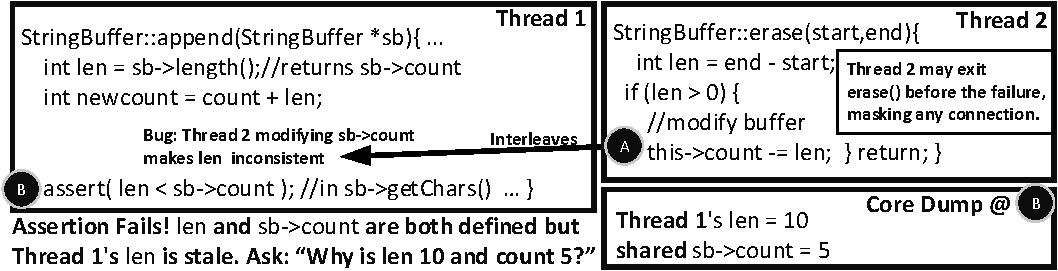
\includegraphics[width=\columnwidth]{figs/JDKStringBufferFail.pdf}
\caption{\label{fig:coreDumpFail}{\bf Atomicity violation bug in a string buffer implementation.} The core dump does not reveal the connection between {\tt append()} and {\tt erase()}, which is crucial to understand the bug.}
\end{figure}

Figure~\ref{fig:coreDumpFail} illustrates the role of provenance information in
debugging, using buggy code from the JDK-1.4 stringbuffer library, adapted to
C++ by other researchers and used variously in prior
work~\cite{concurrencybugs}.  The stringbuffer object pointed to by {\tt sb} in
Thread 1's code contains a buffer and a variable called {\tt count} that stores
its length.  The {\tt append()} code should atomically read {\tt sb->count} and
update the string's buffer (the full update code is not pictured).  The failure
occurs when the {\tt append()} code in Thread 1 is interleaved with the {\tt
erase()} code in Thread 2 as indicated in the figure.  The {\tt erase()} code
updates the buffer's {\tt count}, making the version that Thread 1 read into
{\tt len} stale.  Thread 1's assertion fails at {\bf B} using the stale {\tt
len} value, causing a crash.  

When the failure manifests, Thread 1 is at the assertion in {\tt append()}, as
pictured.  However, Thread 2 may have completed its erase operation and moved on
to execute some unrelated code.  The call stack for Thread 2 may show nothing
about its involvement in the failure, despite the fact that its interleaving
with the {\tt append()} code is the root cause.  Examining the core dump, the
programmer can see that the length and buffer are inconsistent, but is left to
ask {\em why} they are inconsistent.  

Understanding the connection between {\tt append()} and {\tt erase()} is the
key to fixing this bug.  The provenance of the value stored in {\tt sb->count}
at {\bf B} was the write at {\bf A} in {\tt erase()}.  Provenance information
shows the programmer that key connection.  Prior provenance work on origin
tracking for unusable values~\cite{badapples} does not help here.  The involved
values are inconsistent, but they are all {\em usable} so their provenance
would not be tracked.   

Another challenge posed by this bug is that it manifests as a failure
infrequently and under only real-world conditions.  Prior slicing and
provenance debugging
techniques~\cite{tipslicingsurvey,thinslicing,whylineicse}, have overheads too
high to use in production.  Used offline, these techniques may not observe the
failure in a reasonable amount of time and triggering the bug may require
unavailable real-world inputs making offline analysis impossible.   A better
strategy is to continuously collect that information in deployed systems and
package it with core dumps sent to programmers with bug reports.  In this work,
we propose a last writer slicing design that espouses this {\em in situ} data
collection strategy and does so with overheads appropriate for production
systems.


\subsection{Communication Tracking in Concurrency Analyses}
\label{sec:background:comm}

Many useful concurrency analyses rely on monitoring inter-thread
communication.  The domains of these analyses include 
debugging~\cite{defuse,conseq,recon,bugaboo,raceslicing,fasttrack,falcon},
software engineering~\cite{oshajava,oshatr}, anomaly
detection~\cite{avio,dmtracker,cci,daikon}, bug and failure
avoidance~\cite{aviso,cfix} and concurrent performance
profiling~\cite{threadcriticality,schedpredictionmodel}.  The breadth of
applications illustrates the generality of communication tracking.

Despite the potential of a general communication tracking mechanism, prior work
has largely relied on {\em ad hoc} communication analyses.  For example,
DefUse~\cite{defuse} tracks communication via read-after-write (RAW)
dependences, but not write-after-write (WAW) dependences.  Recon~\cite{recon}
tracks some inter-thread WAW and RAW dependences.  These analyses could both be
built with a general communication tracking mechanism.  Unfortunately, their
single-purpose implementations track slightly different information, making
them incompatible and difficult to compose.

These analyses vary in their purpose and environments, but a cross-cutting
theme is the advantage reaped from their use in a deployment environment.
Debugging tools, profilers, and anomaly detectors benefit from seeing diverse,
real-world behavior.  Dynamic failure avoidance techniques must work in
deployed systems to be effective.  Deployment environments demand low overheads
and all of these analyses benefit from a general, high-performance
communication tracking framework.  Unfortunately, many of these techniques are built using heavy-weight infrastructure, like binary instrumentation~\cite{pin}, with overheads too high for production.  

There is a need for a general communication tracking framework that has
performance overheads that are low enough to use in production systems.  As we
describe in Section~\ref{sec:ctraps}, we aim to satisfy that need in this work.



%For example, in a software transactional memory (STM) system~\cite{stm}
%communication corresponds to interference between accesses in different threads
%that must be detected to rollback conflicting transactions.  Deterministic
%concurrent runtime systems~\cite{coredet,grace} similarly monitor
%communication, to apply deterministic ordering constraints.  STMs and
%deterministic systems must track all dependences and they must track them
%precisely, to provide strong guarantees as programming and execution models.
%Unfortunately, precision has a high runtime overhead -- {\em e.g.}, CoreDet
%incurs a mean overhead of around 5x~\cite{coredet}.  This overhead is too high
%for use in production.  





\section{Last Writer Slices}
\label{sec:lastwriterslices}
A last writer slice is a dynamic property of a memory location at a point in a
program's execution.   A memory location's last writer slice is a record
containing the program point and the identifier of the thread that last wrote
data to that memory location.  


We gather last writer slices at runtime by maintaining a {\em last writer
table} (\lwt) that maps from a memory location's address to its last writer
slice.  Just before a thread writes to a memory location, the thread first
finds the memory location's entry in the \lwt and updates that entry with its
thread identifier and its current point in the program.  After updating the
\lwt, the thread performs the original memory access.  


Figure~\ref{fig:basicLWT} shows the basic operation of the \lwt.  The right
side of the figure shows a program execution with three threads.  On the left
is the \lwt at the point of each memory access.  There are three key things to
notice.  First, write operations update the \lwt entry of the memory location
they access.  Second, there is no action necessary for read operations.  Making
read operations cheap is key to making the overhead of last writer slicing low
enough for production use.  Third, if the program stops at a point like the
{\tt Rd Y} illustrated in Thread 1, the \lwt holds provenance information for
the involved values ({\em i.e.}, Thread 3 last wrote {\tt Y} at the code point
shown). That information helps understand {\em why} {\tt Y} holds its value.


\begin{figure}[h]
\centering
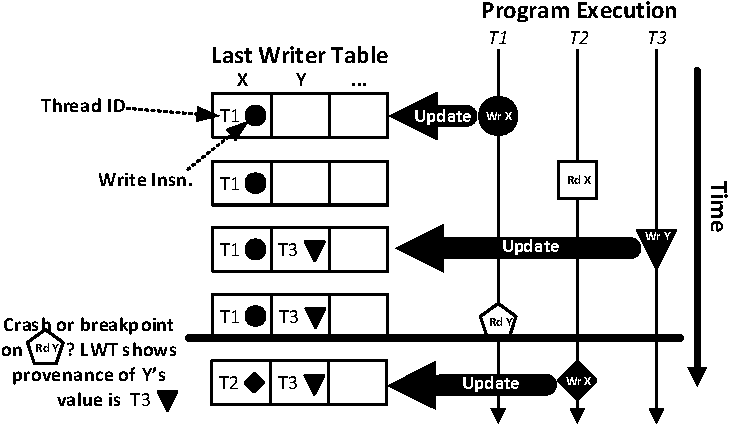
\includegraphics[scale=.6]{figs/BasicLWT.pdf}
\caption{\label{fig:basicLWT}Basic operation of the last writer table. Different shapes signify different distinct memory operations. }
\end{figure}


\subsection{Debugging with Last Writer Slices}
\label{sec:debugging}
%To answer data provenance questions during debugging, prior work has mostly
%used dependence slices that include intra-thread
%dependences~\cite{whylineicse,conseq,tipslicingsurvey}.  The overhead of
%slicing dependence chains and tracking temporal sequences is often high,
%relegating such techniques to working on traces~\cite{whylinechi} or debugging
%executions run ``in the lab''.  

At each point in an execution, a memory location's \lwt entry represents the
provenance of the data stored in that memory location.   Last writer slicing
performs no action on read operations and to be useful, it does not need to.
Instead, a programmer can examine an \lwt entry at any arbitrary point in an
execution and see a value's
provenance ({\em e.g.}, at a breakpoint or after a failure).  Including the \lwt with core dumps means provenance is available
when post-mortem debugging production failures.

Figure~\ref{fig:jdklws} illustrates how the information in the \lwt helps debug
the JDK stringbuffer bug introduced in Figure~\ref{fig:coreDumpFail}.  Recall
that the failure occurs because Thread 2's execution of {\tt erase()} violates
the atomicity of Thread 1's execution of {\tt append()}.  The \lwt entry for
{\tt sb->count} at {\bf B} shows the programmer that its last writer was Thread
2 at {\bf A}. Thread 2 may have run ahead to an arbitrary point in its
execution.  Nothing in the core dump implicates {\tt erase()} in causing
this bug.  The last writer slice reveals the interference between {\tt append()}
and {\tt erase()} via {\tt sb->count}, helping the programmer understand the
bug's cause.


%The core dump does not provide any
%insight into why the mutex is invalid at the time of the call or what its
%value should have been instead.


\begin{figure}[h]
\centering
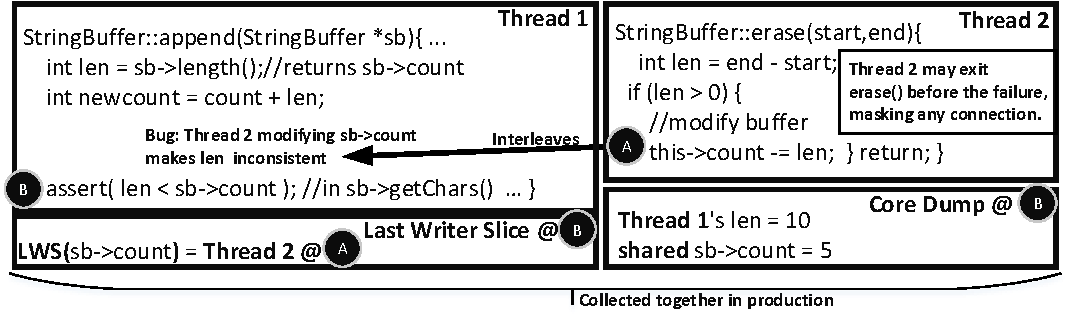
\includegraphics[width=\columnwidth]{figs/JDKStringBufferDebug2.pdf}
\caption{\label{fig:jdklws}{\bf Using last writer slices to debug an
ordering violation in the JDK 1.4 StringBuffer library.} The last writer slice reveals the buggy interaction between {\tt erase()} and {\tt append()}.}
\end{figure}


Another important trait of last writer slices illustrated by
Figure~\ref{fig:jdklws} is that when the assertion fails at {\bf B}, stopping
the execution, the \lwt is saved and can be sent to the programmer with the
core dump.  Capturing good debugging information is especially important for
concurrency bugs that manifest very rarely or in the presence of only peculiar
real-world inputs.  A primary goal of this work is to show that we can collect
last writer slices with very low overheads so they can be included pervasively
in bug reports.

%We discuss last writer slices in more depth by first describing our run time
%support for collecting them.  The system support consists of a runtime library
%and a compiler analysis.  Section~\ref{sec:debugging} shows how last writer
%slices help with debugging using our running example from
%Figure~\ref{fig:bgcoredumpfail}.  We formalize last writer slices in
%Section~\ref{sec:lwssoundness}.

\subsection{Runtime \& Compiler Support}

Figure~\ref{fig:lwsoverview} shows an overview of our system support for last
writer slicing.  The programmer writes their program as usual. Our compiler
instruments write operations in the program with calls to our runtime that
update the \lwt.  The \lwt is maintained in the runtime and saved for use
during debugging, like the core dump. 

\begin{figure}[h]
\centering
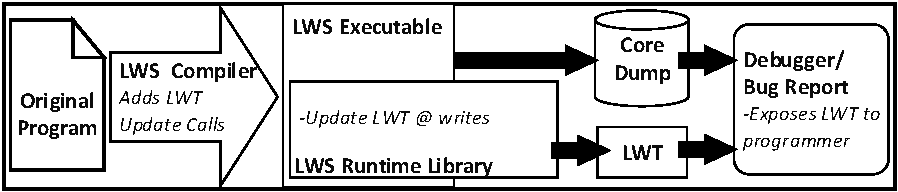
\includegraphics[width=.9\columnwidth]{figs/LWS_Overview.pdf}
\caption{\label{fig:lwsoverview}{\bf Overview of system support for last writer slicing.} Our compiler and runtime library ensure the \lwt remains updated so it can be used during debugging.}
\end{figure}

The \lwt implemented in the runtime library is a {\em shadow memory} that holds
one entry for each potentially shared memory address accessed by the program.
Each \lwt entry records the thread and program point that last wrote to the
entry's corresponding memory location.  When a thread performs a write to a
memory location, our runtime library's \lwt update function updates the \lwt by
recording the thread's identifier and the program point of the write operation
in the memory location's \lwt entry.  A program point may be an instruction
address or a call stack.  We use instructions by default, but we also experimented
with 2-address call stacks.   

Collecting last writer slices requires instrumentation on each write operation.
We built an instrumenting compiler pass that inserts a call to the \lwt update
function in our runtime library just before each write that may access data
last written by another thread (escaping memory accesses).  \lwt update 
calls are passed three pieces of information: the address of
the memory word involved in the access, the thread identifier of the accessing
thread, and the accessing program point.   We use a {\tt GCC}'s local function
escape analysis to identify accesses to memory locations that are provably
inaccessible to code running in other threads.  Such operations access unshared
data and we do not instrument them.  

%Using an inter-procedural thread escape analysis may eliminate more
%instrumentation sites.  


\subsection{\lwt Formalism and Correctness}
\label{sec:lwssoundness}
To discuss the correctness of our \lwt-based last writer slice support, we
first develop a formal description of last writer slices.  We consider an
N-threaded program $P = \{P_1, P_2, \ldots P_N\}$, where $P_t = (p^{t}_{1},
p^{t}_{2}, \ldots, p^{t}_{k_{t}})$ is the sequence of $k_{t}$ dynamic
instructions executed by thread $t$.  Without loss of generality, we assume all
instructions are memory reads and writes, with the form $Op(m)$ where $Op$ is
$Read$ or $Write$ and $m$ is a uniquely addressed memory location.
A point in an execution of $P$ after $e$ instructions have
executed is defined by $Q = (q_{0}, \ldots, q_{e})$ where each $q_{i} \in Q$ is a
$p^{t}_{j}$ from one of the $k_t$ instructions of thread $t$.  We introduce
$LWS[m]$ -- the Last Writer Slice for memory location $m$.   At any point $Q$,
$LWS[m]$ holds $(t,p^{t}_{\ell w})$, where $p^{t}_{\ell w} = max_{\ell}( 
q_{\ell} = Write(m) \in Q)$ and $t$ is the thread that
executed $p^{t}_{\ell w}$. Informally, $p^{t}_{\ell w}$ is the last instruction
in $Q$ to write $m$ and $t$ is the thread that executed it.  For an
unwritten location $n$, $LWS[n] = (\emptyset,\emptyset)$.

For our design to be correct, $LWT[m]$, the entry for a memory location $m$ in
our \lwt implementation, must be the same as $LWS[m]$ at all points in an
execution.  Correctness in the \lwt requires {\em soundness} and {\em
completeness}.  A {\em sound} design updates $LWT[m]$ only when $m$ is written.
A {\em complete} design always updates $LWT[m]$ when $m$ is written.  Our
compiler inserts \lwt updates before every write operation (for completeness)
and only before write operations (for soundness).  Formally, given a program,
$P$, our compiler pass transforms it to a new program, $P'$.  Each thread in
$P'$ executes a modified sequence of instructions: $P'_{t} \in P' = ( 
I(p^{t}_{1}), p^{t}_{1}, \ldots, I(p^{t}_{k_{t}}), p^{t}_{k_{t}} )$.
$I(p^{t}_{j})$ sets $LWT[m] = (t,p^{t}_{j})$ if and only if $p^{t}_{j} =
Write(m)$ and is a no-op otherwise.  This reasoning shows our \lwt is both
sound, complete, and thus correct.

Next we discuss two nuances of our design: (1) the interaction of our \lwt
implementation with data-races; and (2) the correctness of the
\lwt for accesses to overlapping memory regions. 

\paragraph{Consistency and Atomicity}

Our implementation of the \lwt does not add any synchronization to the program.
As a result our analysis does not incur the overheads or possible thread
schedule perturbation synchronization can cause.  However, there are two
potential issues that stem from this design choice. First, we do not enforce
memory consistency of meta-data reads and writes in different threads.  Second,
our implementation does not enforce the atomicity of \lwt updates and their
corresponding program accesses.  In the absence of data-races our \lwt
implementation is {\em always correct} and neither of these issues exist.  Both
atomicity and ordering is enforced by the program synchronization that ensures
consistency for program data.   

We use our \lwt formalism to show that without data-races, \lwt updates and
their corresponding memory accesses are atomic and well-ordered.  The relation
$p \prec q$ denotes that $p$ happens before $q$.  In correctly synchronized
code, any write by thread $t$ to $m$, $p^{t}_{j} = Write(m)$, is ordered by
program synchronization with $p^{t'}_{j'} = Op(m)$, a later access to $m$ by
any other thread $t'$ -- {\em i.e.}, $p^{t}_{j} \prec p^{t'}_{j'}$.  Our
compiler inserts an \lwt update $I(p^{t}_{j})$ into $P'$ before its write
operation, $p^{t}_{j}$. Thus, $I(p^{t}_{j}) \prec p^{t}_{j}$ due to program
order.  $I(p^{t'}_{j'})$ is inserted before $p^{t'}_{j'}$, but after the synchronization that orders $p^{t'}_{j'}$ and $p^{t}_{j}$, so $p^{t}_{j} \prec I(p^{t'}_{j'})$.  Happens-before is transitive, so without data-races, $I(p^{t}_{j})
\prec p^{t}_{j} \prec I(p^{t'}_{j'}) \prec p^{t'}_{j'}$, meaning $I(p^{t}_{j})$
happens before all accesses that $p^{t}_{j}$ happens before {\em and before
their respective \lwt updates}, $I(p^{t'}_{j'})$.  Symmetrically, for any
access $p^{t''}_{j''}$ in another thread $t''$ that precedes $p^{t}_{j}$,
$p^{t''}_{j''} \prec p^{t}_{j}$.  Our compiler inserts each $I(p^{t}_{j})$
immediately before each $p^{t}_{j}$, so $I(p^{t''}_{j''}) \prec p^{t''}_{j''}
\prec I(p^{t}_{j}) \prec p^{t}_{j}$, happens-before ordering $I(p^{t}_{j})$
after all preceding accesses to $m$ in other threads, {\em and after their
repective \lwt updates}.  Thus, at all points $Q$ in a data-race free
execution, given $q_r = I(p^{t}_{j})$, $q_p = p^{t}_{j}$, and $q_r \prec q_p$,
$\forall_{ \{q_s | q_r \prec q_s \prec q_p \}}: q_s \ne Op(m) \wedge q_s \ne
I(Op(m)) $.  In other words, \lwt updates and their accesses are atomic.

In a program with a data-race, there are some accesses, $p^{t}_{j}$ and
$p^{t'}_{j'}$, that are concurrent.  The \lwt updates for these accesses are
also concurrent because they are not transitively ordered by the accesses' ordering.  The unordered accesses and \lwt updates can interleave arbitrarily
because they are concurrent.  Some racy thread schedules may violate the
atomicity of accesses and their \lwt updates.  Such an execution could reach a
state $Q_{bad} = (\ldots, I(p^{t}_{j}), I(p^{t'}_{j'}), p^{t'}_{j'}, p^{t}_{j},
\ldots)$ and in that state, $LWS[m] = (t,p^{t}_{j})$, but $LWT[m] =
(t',p^{t'}_{j'})$.  The \lwt was effectively not updated when $p^{t}_{j}$
executed (violating completeness), or was effectively updated to reflect that
$p^{t'}_{j'}$ was $m$'s last writer, when $p^{t}_{j}$ was (violating
soundness).    

According to the C++11 language specification, in the presence of a data-race,
a program's behavior is undefined and arbitrary state corruption can occur.  In
the presence of data-races, {\em any} analysis, including our \lwt analysis,
running on such a program could experience arbitrary corruption.  In practice
({\em e.g.}, on x86) these atomicity violations may cause limited \lwt
corruption, but even this is unlikely.  These atomicity violations only occur
only when accesses to the same data occur within a very short time interval,
which is uncommon, {\em and} an unserializable interleaving of accesses and
\lwt updates also occurs.

\paragraph{Non-overlapping Memory References} 
We assume written memory locations do not overlap in memory because our \lwt
design is {\em granularity oblivious}.  We discuss this issue informally due to
space constraints.  Each \lwt entry corresponds to a location that was written.
Two instructions might reference different locations that overlap because the
referenced locations have different granularities ({\em e.g.}, accessing a byte
that is part of a previously accessed word).  When that happens, both accesses
update different \lwt entries, because they reference different locations.
However, the overlapping region then has two different entries reflecting the
last {\em two} updates to its parts rather than just its last write.

The \lwt remains correct, assuming the program only accesses non-overlapping
regions.  In programs that access overlapping regions, there is always some
entry in the \lwt that correctly reflects each memory location's last writer.
However, the coarse region's entry may be stale because of an
access to an overlapping region.

One approach to mitigating this issue would be to allocate \lwt entries for
regions of fixed granularity.  We chose not to do so for two reasons.  First,
associating \lwt entries with regions of  large granularity only ({\em i.e.},
cache-line) precludes sound analysis for fine-grained accesses.  Second,
associating \lwt entries with regions of small granularity ({\em i.e.}, byte)
requires multiple \lwt updates for larger granularity accesses, increasing
their overheads proportionately to the granularity of the access.





\section{Communication Traps}
\label{sec:ctraps}

\ctraps is a framework for analyzing and interposing on inter-thread
communication events during a program's execution.  We build \ctraps on top of
last writer slicing that we described in Section~\ref{sec:lastwriterslices}.
Using last writer slice information, \ctraps dynamically tracks 
inter-thread communication events. \ctraps exposes communication
events as {\em traps} during an execution that {\em trap handlers} can handle
to perform analysis and interposition.  

\subsection{\ctraps Design}

We now discuss \ctraps in more detail by describing the design of our \ctraps
system support.  Figure~\ref{fig:systemdiagram} shows an overview of our system
support.  The programmer writes their program as usual.  They compile it using
the \ctraps compiler. The \ctraps compiler includes the compiler support for
collecting last writer slices.  In addition, the \ctraps compiler also inserts
calls to the \ctraps runtime at points where communication may occur.  The
resulting compiled executable links to the \ctraps runtime that collects last
writer slices and monitors communication.  The runtime loads and manages \ctraps
handlers when the execution starts via a plugin interface.  \ctraps handlers,
written independently of the original program implement \ctraps applications.
Traps are delivered to handlers by the runtime when operations communicate.
Together, the \ctraps executable and the \ctraps handlers are deployed.


\begin{figure}[htb]
\centering
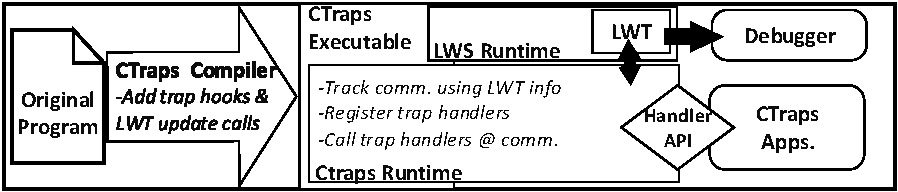
\includegraphics[width=.90\columnwidth]{figs/CTraps_Overview.pdf}
\caption{\label{fig:systemdiagram}{\bf CTraps system support.}}
\end{figure}


%Our system support for \ctraps incorporates the support for collecting last
%writer slices described in Section~\ref{sec:lastwriterslices}.  In addition,
%our \ctraps system support also monitors all read and write operations that
%might communicate and traps on all those that communicate.  

\subsubsection{Compiler and Runtime Support} 

\ctraps delivers software traps before all read and write operations executed
by one thread that access a memory location that was last written by another
thread, {\em i.e.}, communicating memory operations.  Traps are simply inserted
function calls (as opposed to, {\em e.g.}, signals) made before such operations
execution.  \ctraps implements traps using a combination of compiler and
runtime library support.   

\paragraph{Compiler Support}
Our compiler inserts a call to the \ctraps~{\em trap hook} function immediately
before all read and write operations that access potentially escaping memory
locations.  Trap hooks are passed the address of the memory location being
accessed, the thread identifier of the accessing thread, the type of operation
being performed, and the program point of the access.  

\paragraph{Runtime Support}
The \ctraps runtime implements the trap hook function,  which has two purposes.
The trap hook function detects communication and delivers traps to \ctraps
applications when communication occurs.  The trap hook function detects
communication by looking up the \lwt entry for the memory location being
accessed.  If the thread identifier in the \lwt entry is different from the
accessing thread, then the trap hook function delivers a trap to the accessing
thread, just before the memory access is allowed to proceed.  To deliver a
trap, the trap hook function calls {\em trap handler routines} that are defined
in \ctraps applications.  Trap handler routines are like signal handlers.  The
\ctraps runtime maintains a list of trap handlers that are registered when the
program starts via a configuration stored in the environment.  Trap handlers
may contain arbitrary application-specific code.  \ctraps defines a trap
handling API.  Trap handlers are passed the four pieces of information passed
to the trap hook, as well as the \lwt's record of the program point and thread
identifier of the last write to the involved location.

%\begin{figure}[htb]
%\centering
%\begin{verbatim}
%void trap(AccessType type, 
%          ThdId currThd, ProgPt currPt,
%          ThdId lastThd, ProgPt lastPt);
%\end{verbatim}
%\caption{\label{fig:hookapi}The \ctraps trap handling interface.}
%\end{figure}


%MAYBE PUT THIS BACK IN
%\subsection{Formalism and Correctness}
%\label{sec:ctsoundness}
%To discuss the correctness of \ctraps, we first formalize trap delivery by
%building on our last writer slicing formalism from
%Section~\ref{sec:lastwriterslices}.  
%
%Given a program $P'$ already instrumented with \lwt updates, the \ctraps
%compiler produces $P''$. A thread $t$ in $P''$ executes a modified instruction
%sequence, $P''_{t} = \{ T(p^{t}_{j}), I(p^{t}_{1}), p^{t}_{1},$ $\ldots,
%T(p^{t}_{j}), I(p^{t}_{k_{t}}), p^{t}_{k_{t}} \}$, where $T(p^{t}_{j})$ is a
%trap hook call.  We consider a point $Q = \{q_1, \ldots, q_{e-2}\}$ after $e-2$
%instructions of an execution have executed and $q_{e} = p^{t}_{j}$ is about to
%execute after its trap hook $T(p^{t}_{j})$ and \lwt update $I(p^{t}_{j})$
%execute.  The trap hook $T(p^{t}_{j})$ {\em delivers} a trap before if $LWT[m]
%= (t',p^{t'}_{\ell w})$ and $t \ne t'$.  Informally, the trap hook delivers a
%trap before the instruction if the thread that last wrote $m$ is different from
%the one executing the instruction.  When a trap hook, $T(p^{t}_{j})$, delivers
%a trap, thread $t$ executes an arbitrary trap handler $H = \{h^{t}_{1}, \ldots,
%h^{t}_{h_{n}}\}$.  Thus, after the trap, the \lwt update, and the instruction
%execute, the execution reaches the new point $Q = (q_{1}, \ldots, T(q_{e}),
%h^{t}_{1}, \ldots, h^{t}_{h_{n}}, I(q_{e}), q_{e})$, and continues.
%
%A \ctraps implementation must be sound and complete to be correct.  A design is
%{\em sound} if it only delivers a trap when threads have communicated.  A
%design is {\em complete} if it always delivers a trap when threads have
%communicated.  The \ctraps compiler puts a trap hook on all read and write
%operations, and only on those operations.  Assuming a correct \lwt, \ctraps is
%correct.  Our \ctraps implementation also does not insert any synchronization
%into the program, so it comes with the same caveats related to data-race
%freedom as the \lwt.  The same arguments for \lwt correctness apply to the
%correctness of trap delivery and handling.  Most importantly, data-race freedom
%implies that trap hooks, \lwt updates, and accesses are all atomic.


%\paragraph{Escape Analysis}
%All our designs eliminate instrumentation on accesses to memory locations
%statically guaranteed to be inaccessible to other threads.  Doing so has no
%effect on soundness or completeness because accesses to such locations are
%guaranteed never to be communicating.


\subsection{\ctraps Applications}
\label{sec:apps}
\ctraps applications are implemented as shared library plugins that are loaded
by our runtime.  They must implement the \ctraps trap handler API, which
requires a trap handler function and permits a constructor, destructor, thread
constructor, and thread destructor, which allow initialization and disposal of
global and thread-local state.  Many useful \ctraps applications are possible,
several of which were outlined in Section~\ref{sec:background:comm}.    To
demonstrate that \ctraps can implement real analyses with little work, we
implemented two applications. The first application is a version of a debugging
analysis from CCI~\cite{cci}.  The second application is a communication graph
collector, similar to DefUse~\cite{defuse}, Recon~\cite{recon}, and
DMTracker~\cite{dmtracker}.

\paragraph{CCI-Prev Implementation}
CCI-Prev is a technique from CCI~\cite{cci} that records a set of code points
that access a memory location when the previous access to the same location was
by a different thread.  We implemented a variant of CCI-Prev using \ctraps that
records such a set of code points.  In our implementation, communcating read
operations update the LWT like writes normally do.  Under this policy, any
operation that accesses a location that was last accessed by a different thread
is recorded.  The set of recorded accesses is the output of the analysis.  Our
\ctraps implementation of CCI-Prev took about 10 lines of code (on top of our
base system). 

\paragraph{Communication Graph Implementation}
Communication graphs are the basis of several prior debugging
techniques~\cite{recon, bugaboo, defuse}.  We implement communication graph
collection using \ctraps.  When a trap is delivered, our implementation records
communication graph edges composed of the code point of the last writer to the
location being accessed and the code point of the trapping access.  The set of
recorded edges is the tool's output.  Our \ctraps implementation of
communication graphs took about 50 lines of code. 

%\paragraph{Other Applications}
%In addition to those applications, we envision that a variety of applications
%will be enabled by our simple interface.  Anomaly detection and ``likely
%invariant'' techniques similar to AVIO~\cite{avio}, Daikon~\cite{daikon}, and
%others are a natural fit for \ctraps.  \ctraps provides the support necessary
%for implementing specification checkers for specifications related to
%inter-thread communication~\cite{velodrome,oshajava}.  Guided testing
%tools~\cite{cuzz,chess} and bug detection tools~\cite{ctrigger} focused on
%concurrency could also be implemented as \ctraps applications.  \ctraps also
%provides an interesting platform for developing new approaches to
%record/replay~\cite{chimera,fdr}.  \ctraps is an enabling platform for
%developing these or other analyses with low baseline overheads and without the
%need to build an entire concurrency analysis from scratch.

\section{System Implementation}
\label{sec:implementation}
We implemented last writer slicing and \ctraps.  We built our compiler support
as a plugin for GCC ({\tt gcc-4.7}).  We used GCC's points-to and
escape analysis support to prune instrumentation on accesses to non-escaping memory
locations.  Our compiler instruments calls to {\tt free} and {\tt delete} as
writes to the pointer being deallocated.  Our analysis handles all code
compilable using this version of GCC except for a few cases: we do not handle
accesses that compile to GCC {\tt BITFIELD\_REFERENCE} IR types because these
are undocumented, we do not handle inlined assembly instructions, and we do not
handle C++ exceptions.  Note that these limitations of our research prototype
are not fundamental and the limited cases are uncommon.   

We built our runtime system from scratch.  The LWT is a fixed size 2GB array of
64-bit words.  Each entry packs a program point and a thread identifier into
the 64-bit word.  By default, program points are single instruction addresses,
but we also support limited (2-address) context-sensitivity by packing the
current instruction's address and the nearest return address into a 64-bit LWT
entry. When an access to a memory location occurs, we index into the LWT with
the lower bits of the location's address.  Our prototype implementation uses a
lossy resolution policy for hash collisions.  We use this policy in our
prototype because it is fast and bounds memory overheads at 2GB.  Collisions
are rare (see Section~\ref{sec:eval:performance:collisions}), so this
simplification is unlikely to be a problem.  

\subsection{Release}
We released our implementation, free and open-sourced, on the
web~\cite{ctrapsrelease} and published it to the GCC plugin repository.
Since its release, we have seen contributions to our codebase from members of
the GCC community and downloads from interested developers.

\section{Evaluation}
\label{sec:eval}
We evaluated last writer slices and \ctraps along several axes.  We show that
last writer slices provide information that is useful during debugging in
Section~\ref{sec:eval:debugging}, looking at a set of buggy programs and
comparing to prior work.  We evaluate our performance overheads and
show that last writer slices and \ctraps are feasible for use in deployed
systems for a majority of workloads we studied.  We then characterize our
instrumentation and discuss sources of run time overhead.   We
show that \ctraps is useful by implementing two existing applications and
analyzing their performance.    

\subsection{Debugging with Last Writer Slices}
\label{sec:eval:debugging}

We illustrate the debugging benefits of last writer slices by using our system
to debug several real-world programs studied previously in the debugging
literature.  Table~\ref{tab:bugs} provides an overview of this evaluation and
Section~\ref{sec:eval:debugging:cases} looks in detail at several cases to 
better illustrate how last writer slices helps with debugging.

In Table~\ref{tab:bugs}, we show the bugs we studied, describing the program,
bug type, and bug report identifier where applicable.  For each bug, we
followed the procedure for installation and bug triggering described by the
author of~\cite{concurrencybugs}.  We study a mixture of concurrency bug types
in this work, including both single- and multi-variable bugs and both atomicity
and ordering violations.

The table also summarizes our evaluation of last writer slicing's debugging
benefits.  We mirror the evaluation strategy of bad value origin
tracking~\cite{badapples}, as it is the only other low-overhead provenance
tracking mechanism we know of.  We evaluate our system using their three
evaluation criteria - (1) {\bf effectiveness}, (2) {\bf triviality}, and (3)
{\bf usefulness}.  Our technique is {\bf effective} if it tracks a correct last
writer slice for the value or values involved in causing the failure.  A failure is {\bf
trivial} to debug if its cause is made obvious by examining the core dump
alone, {\em i.e.}, a last writer slice is unnecessary.  A last writer slice is
{\bf useful} if it is effective and the thread and code point in the slice help
understand why the failure occurred or how to fix it.   We directly compare to
bad value origin tracking~\cite{badapples}.    The {\bf O.T.} column in Table~\ref{tab:bugs}
shows  whether their analysis could help debug each bug, based on the
description of their technique.

\begin{table}
\scriptsize
\centering
\begin{tabular}{l|ll|l|ccc|c}
{\bf App} & {\bf Ver. \#} & {\bf Bug \#} &{\bf Type} & {\bf Eff.?} & {\bf Triv.?} & {\bf Usef.?} & {\bf O.T.?}\\ \hline
jdk1.4 &  1.70   &  N/A     & Atom.  &Yes  &No    &Yes   & No  \\%All values usable
pbzip2 &  0.9.4  &  N/A     & Order  &Yes  &No    &Yes   & Yes \\
httrack& 3.43.9  &  N/A     & Order  &Yes  &No    &Yes   & No  \\%Used w/o origin - no help
transmission & 1.42 & N/A   & Order  &Yes  &No    &Yes   & No  \\
mysql  &  4.0.12 &  791     & Atom.  &Yes  &No    &Yes   & No  \\%All values usable
apache1&  2.0.48 &  21285   & Atom.  &Yes  &No    &Yes   & Some \\%All values usable
apache2&  2.2.9 &  45605    & Atom.  &Yes  &No    &Some  & No \\%All values usable
\end{tabular}
\caption{\label{tab:bugs}{\bf Concurrency debugging with last writer slices.} We describe each bug and summarize the debugging benefit of last writer slices using the evaluation criteria from ~\cite{badapples}.  }
\normalsize
\end{table}

The results in Table~\ref{tab:bugs} show that for both atomicity and ordering
violation bugs, last writer slices are effective.  In all cases, we found that
the last writer slice revealed the provenance of at least some data involved in
the failure, so last writer slicing was effective.  We found that none of the
failures we looked at were trivially debuggable.  This finding is consistent
with the difficulty of debugging concurrency bugs -- the core dump does not
reveal the interaction between threads that led to a failure, only the result
of the interaction.  

Last writer slices were useful for helping understand how to fix the bug in
all but one case and useful at least for understanding the bug in the
remaining case, {\tt apache2}.  The main reason last writer slices are helpful
is that they reveal the connection between code running in different threads
that interacts to cause a failure.  Without last writer slices, programmers
have no easy way of connecting these otherwise disparate parts of a program.
The case studies in Section~\ref{sec:eval:debugging:cases} show in more detail
how last writer slices are useful for debugging and illustrate their limitations.


%For the remaining case, {\tt apache2}, last writer slices would
%probably help with debugging, but it is less obvious because this bug is a
%complex, multi-variable bug.  We provide more detail on {\tt apache2} in
%Section~\ref{sec:eval:debugging:cases}.
Our evaluation shows that bad value origin tracking~\cite{badapples} is
helpful in one case where last writer slices is useful and provides limited help
in one other case.  For a use-after-delete bug in {\tt pbzip2}, bad value
origin tracking helps.  For this bug, when one thread deletes a variable, it
makes that variable unusable and bad value origin tracking would track that
value.  When the failure occurs, the programmer would then know why the value
was deleted.  

For {\tt apache1}, bad value origin tracking may help.  The bug is an atomicity
violation that leads to a double free.  Two threads manipulate an object's
reference count and deallocate the object when the count hits zero. Zero-checks
and deallocation should be atomic, but the code does not ensure they are.  If
threads interleave their code, multiple threads might see zero reference
counts, which is incorrect.  When that happens, both threads try to free the
object and the second free causes a crash.  

Bad value origin tracking may help in this case.  At the first free, the freed
pointer becomes unusable and its origin is tracked.  At the crash, the bad
value's reported origin is the code point of the free. That information may
help debug the program by suggesting a double free.  However, in {\tt apache},
many threads perform different tasks and all call the same free code.  Bad
value origin tracking does not record the thread information.  The programmer
is left unsure whether the problem is with single-threaded logic or
synchronization.  In contrast, last writer slices reports the code point and
thread, making it clear the bug is a concurrency bug and identifying the
involved threads.

\subsubsection{Debugging Case Studies}
\label{sec:eval:debugging:cases}

We now provide detailed cases studies showing the debugging role of last writer
slices in several of the bugs we examined.  

%Space constraints prevent us from providing details for all cases.


\paragraph{jdk-1.4}
The running example in Figures~\ref{fig:coreDumpFail} and ~\ref{fig:jdklws},
and the text in Section~\ref{sec:debugging} describes the benefit provided by
last writer slices in debugging an ordering violation in the JDK-1.4.

%\paragraph{Apache}
%%http://issues.apache.org/bugzilla/show_bug.cgi?id=21287
%%concurrency-bugs
%We conducted a case study using Apache httpd-2.0.48, which has a bug in its
%script cache. The cache uses reference counting to determine when to deallocate
%cached objects.  When a thread sees a reference count hit zero, it frees the
%object.  The bug is that the check that the count is zero and the deallocation
%are not atomic but it should be.  Multiple threads may see the zero reference
%count and free the object more than once, leading to a crash. 
%
%We debugged this issue by examining the core dump from a crashing execution.
%The core dump showed that the memory allocator aborted due to one thread
%freeing already freed memory at {\tt mod\_mem\_cache.c}, line 287.  We examined
%the last writer table entry for the object being freed at that point.  That
%entry revealed that a different thread last wrote that object at the same point
%in the code.  The information in the last writer table illustrates why the
%double free bug is happening -- two threads end up in the object deallocation
%routine for the same object, which should not happen.


\paragraph{httrack}
Figure~\ref{fig:httlws} shows how last writer slices help understand the root
cause of a concurrency bug from HTTrack-3.43.9.  The program crashes at point
{\bf B} when it calls {\tt hts\_mutex\_lock()} with an invalid mutex.    The
root cause of this bug is that Thread 1 fails to initialize the mutex before
Thread 2 uses it.   The core dump is of little debugging use, only showing
that, indeed, the lock is uninitialized.  Even if the programmer compared the
core dump from the failing run to the memory image from a correct execution --
a helpful debugging strategy -- they would find only that in a correct
execution, the lock contains valid mutex state.

\begin{figure}[h]
\centering
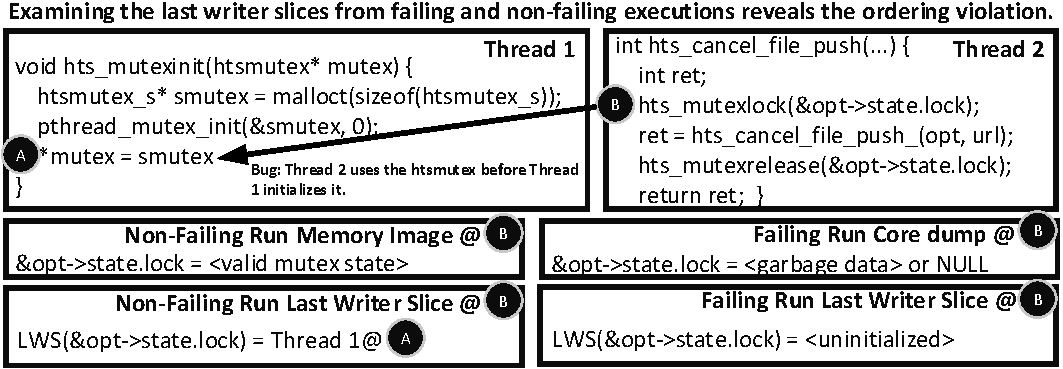
\includegraphics[width=\columnwidth]{figs/LWSHTTDebug.pdf}
\caption{\label{fig:httlws}{\bf Using last writer slices to debug an
ordering violation in HTTrack.} The provenance information stored in the last
writer slice for the mutex variable helps understand the bug's root cause.}
\end{figure}

Looking at last writer slices make this root cause clear: in the failing
execution, the last writer slice indicates the mutex is uninitialized; in the
non-failing execution, the last writer slice indicates the mutex was
initialized by Thread 1 at point {\bf A}. While the core dump provides no
information about the connection between point {\bf A} and point {\bf B}, the
last writer slice reveals that the programmer should ensure {\bf B} follows
{\bf A} to prevent the failure.  Note that even augmenting the core dump with
bad value origin tracking~\cite{badapples} does not help with this bug.  In the
failing execution, origin tracking shows that the unusable lock is
uninitialized, revealing no more than the core dump.  In the non-failing
execution, origin tracking does not monitor the {\em usable} lock value, adding
nothing.  By contrast, comparing the last writer slices for the failing and
non-failing executions reveals how to fix this bug.  


\paragraph{transmission} We used last writer slices to debug a
use-before-initialization bug in transmission-1.42.  We omit a full case study
due to space constraints, but we mention a few notable properties of this case.
First, like {\tt httrack}, we debug {\tt transmission} by comparing the last
writer slice from failing and non-failing executions.  Second, last writer
slices reveal all the code and data involved in this bug, making the bug and
its fix clear.   Third, bad value origin tracking does not work in this case
because in failing executions, the bad value has no origin and in non-failing
executions, the involved variable holds only usable values.

%
%\paragraph{PBZip2}
%We conducted a case study using a buggy version of PBZip2-0.9.1.    The bug is
%a use-after-delete bug that leads to an assertion failure.  A worker thread
%tries to acquire a mutex after it has been deleted by the main thread during
%shutdown, causing the assertion to fail.  
%
%Last writer slices provide the key piece of information to debug this failure.
%When the program fails, the core dump shows that the mutex is invalid because
%it has been deleted.  The mutex's last writer slice shows that the last write
%to the mutex before the worker tried to acquire it was when the main thread
%deleted it.  The last writer slice reveals the connection between the the two
%pieces of code involved in the bug: the code that acquires the mutex and the
%code that deletes the mutex.  Note that this connection is not obvious when the
%program crashes because the main thread may have executed arbitrarily far from
%where it deleted the mutex before the worker thread crashes.  

\paragraph{mysql}

We used last writer slices to debug an atomicity violation in MySQL-4.0.12 that
is a critical security vulnerability.  Figure~\ref{fig:mysqllws} shows the
buggy code.  Thread 1 rotates the database's log file.  Log rotation should be
atomic, but the lack of synchronization allows Thread 2 to run its insert
during log rotation.  In that case, the insert query is not logged, manifesting
the failure.  We added an {\tt abort} statement to the non-logging case because
this behavior is a security vulnerability that the bug report describes as
``critical''.  Adding the {\tt abort} is reasonable, as the bug report
describes the {\tt else} block as an error case.  Running in a debugger, a
programmer might equivalently use a breakpoint, rather than adding an
{\tt abort}.


\begin{figure}[h]
\centering
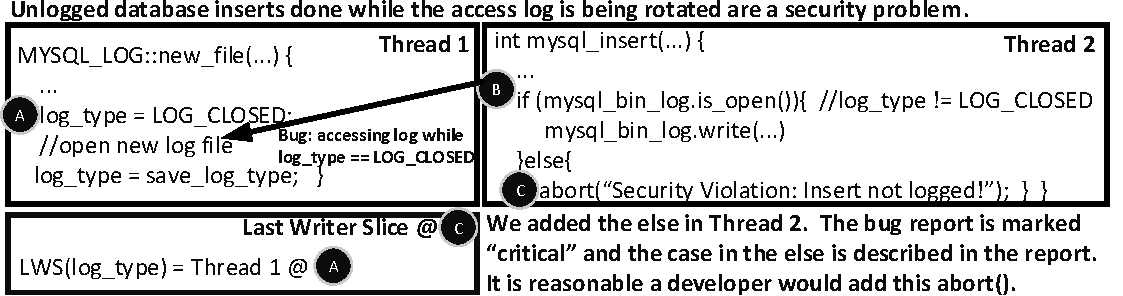
\includegraphics[width=\columnwidth]{figs/MySQLDebug.pdf}
\caption{\label{fig:mysqllws}{\bf Using last writer slices to debug an
atomicity violation in MySQL 4.0.12.} The last writer slice reveals the code that closes the log before a database insertion that goes unlogged, which is a security problem.}
\end{figure}

We triggered the bug by running an insert query during a log rotation and
execution stopped at {\bf C}.  The core dump showed the log was marked closed,
which is the failure state ({\em e.g.}, {\tt log\_type} was {\tt LOG\_CLOSED}).
However, the core dump did not reveal {\em why} the log was marked closed.  The
last writer slice at {\bf C} for {\tt log\_type} shows that it was written last
by Thread 1 at {\bf A}, in the log rotation code, which should be atomic.
Thus, the last writer slice shows the programmer the need for log rotation to
be atomic with respect to the insert code to prevent this failure.  Bad value
origin tracking does not help debug this bug because {\tt log\_type} only ever
contains usable values so it would not be tracked.  

\paragraph{apache2}
We used last writer slices to debug an atomicity violation in Apache-2.2.9 and
we found that last writer slices help understand the bug, but not fully how to fix
it.  The bug involves a group of worker threads that handle web requests and a
network listener thread that passes requests to the workers.  The server tracks
the number of idle workers.  When a worker becomes idle, it increments the
number of idlers and when the listener passes work to a worker, it decrements
that number.  The counter's increments and decrements are synchronized using
condition variables.  If there are no idlers, the listener waits for a signal.
When a worker becomes idle when no others are, it delivers a signal to the
listener.

The problem is that the listener does not check the condition governed by the
condition variable after being signaled on that condition variable.  As a
result, the listener can incorrectly decrement the idler count twice,
underflowing the unsigned value, which then causes an assertion to fail.  When
the failure occurs, the core dump shows the idler count underflowed, revealing
a primary symptom of the bug, but not providing much help.  The last
writer slice for the idler count reports that the listener thread last
wrote the idler count at its decrement operation.  That information shows the programmer
{\em why} the underflow occurred, which is helpful for understanding the
failure.  However, we conclude that last writer slices are only somewhat 
useful in this case.  Solving this complex bug requires understanding not just
the connection between the underflow and the listener's decrement, but also the
synchronization protocol that coordinates that decrement and other accesses to
the variable.  

\subsection{Performance Evaluation: Setup and Benchmarks}

We conducted our evaluation on a machine running Linux 2.6.27-7, with a 2.27GHz
8-core Xeon E5520 processor with 2-way SMT ({\em i.e.}, 16 execution contexts)
and 10GB of memory.  We evaluated our system using PARSEC, a set of
architectural benchmark programs~\cite{parsec} and a collection of real server
and desktop applications.    

\subsubsection{PARSEC}

We ran PARSEC programs with their {\tt native} input set, and with each
program's 8 thread configuration. We have omitted three of the PARSEC
benchmarks because our compiler pass does not handle C++ exceptions.    

\subsubsection{Servers}


\paragraph{MySQL-5.1.65} MySQL is an industrial-strength database
server. To benchmark MySQL, we used {\tt SysBench OLTP} running with its
default 8 threaded configuration, measuring MySQL's performance to be the
throughput reported by {\tt SysBench}.  

\paragraph{Apache-2.4.3} 
Apache-httpd is a popular web server.  To benchmark Apache, we used {\tt
ApacheBench} to request a static {\tt html} page 1,000,000 times using 8
threads, measuring Apache's performance to be the throughput reported by {\tt
ApacheBench}.  

\paragraph{LevelDB-1.5.0}
LevelDB is a carefully tuned high-performance key-value store written by Google
developers. To benchmark LevelDB, we used the included {\tt db\_bench} utility,
running its ``Read while Writing'' test with 8 threads.  We measure LevelDB's
performance to be the operation throughput reported by {\tt db\_bench}.

\paragraph{Memcached-1.4.4}
Memcached is an in-memory key-value store frequently used as a cache for web
services.  We were unable to find a standard benchmark for Memcached.  Instead,
we wrote a C program that uses libmemcached-0.49 to issue a
mixture of 10\% load requests and 90\% store requests for a single key 
simultaneously from 8 threads.  We measured Memcached's performance to be the
total time to complete 10,000 requests in each thread.



\subsection{Performance Evaluation}
\label{sec:eval:perf}

The main performance result of our work is that our designs impose performance
overheads that are low enough for use in deployed systems for many of our
experimental workloads.  Figure~\ref{fig:perfall} shows the slowdown suffered
by our benchmarks due to last writer slicing and \ctraps running with ``no-op''
trap hooks ({\em i.e.}, no handlers), relative to the natively executing
baseline.  In these experiments, we consider a run time overhead of 10\% or
less to be ideal for production use and a run time overhead of 50\% as
a reasonable upper bound on acceptable overhead for production use.

\paragraph{Last Writer Slices}
The data show that last writer slicing has very low overheads with a geometric
mean of less than 10\% across our server programs and less than 50\% across
PARSEC.  Such low overheads are likely to be acceptable in production.  In many
cases (Apache, MySQL, {\tt dedup}, {\tt canneal}), overheads are negligible.
In all but two cases ({\tt vips} \& {\tt swaptions}), the overhead of
collecting last writer slices is less than 100\%.    

\paragraph{\ctraps}
\ctraps imposes a geometric mean overhead of 14\% for server applications and
110\% for PARSEC applications.  In 7 out of 13 of our tests, the overhead of
\ctraps is less than 50\%.  These seven low overhead benchmarks include all of
our server programs, as well as {\tt blackscholes}, {\tt dedup} and {\tt
canneal} from PARSEC.  The overhead for these applications is likely to be
tolerable in production.  {\tt vips} and {\tt swaptions} saw the highest
overheads -- around 400\%.  We discuss sources of high overheads in
Sections~\ref{sec:eval:conservative} and~\ref{sec:eval:parsecserver}.

By comparing \ctraps and last writer slicing, we see four applications ({\tt
dedup}, {\tt streamcluster}, {\tt fluidanimate}, {\tt ferret}) that have
\ctraps overhead that is probably too high for production use (averaging
153\%).  By comparison, those applications have a last writer slicing overhead
that is likely acceptable for production use (averaging 38\%).  The difference
indicates that these programs perform relatively more reads than other
applications, experiencing more overhead due to \ctraps's read instrumentation.

These high-level results support our claim that our overheads 
are low enough for deployed systems for many applications, especially
for servers.  We now further analyze our observed overheads, illuminating
differences between the lower-overhead server programs and the higher-overhead
PARSEC programs.

\begin{figure}
\centering
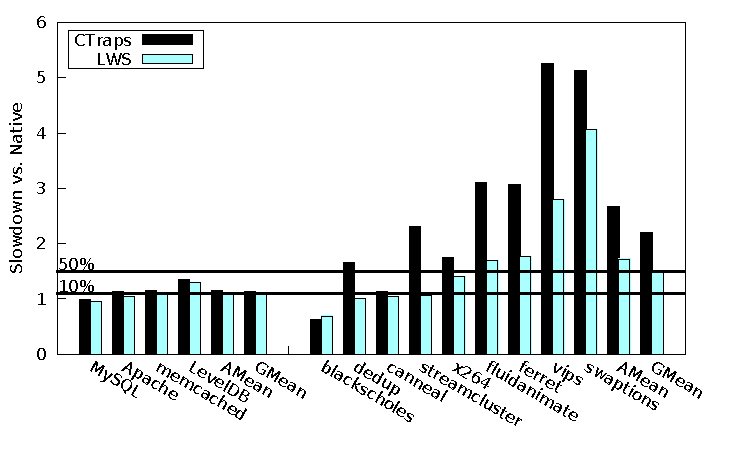
\includegraphics[width=.9\columnwidth]{plots/perf.pdf}
\caption{\label{fig:perfall}Runtime overhead of \ctraps and Last Writer Slices (LWS).}
\end{figure}

\subsubsection{Overheads Due to Conservative Escape Analysis}
\label{sec:eval:conservative}
{\tt swaptions} had the highest run time overhead in our tests.  We
investigated the cause and determined it is largely due to shortcomings in our
escape analysis.  We located the inner-loop function {\tt
HJM\_SimPath\_Forward\_Blocking}.  The function uses two local matrices that
are allocated through an external call.  Our escape analysis cannot determine
that the matrices are only used locally in that function, so it conservatively
assumes the matrices escape.  We manually inlined the matrix allocation calls
(and a matching deallocation calls), and escape analysis eliminated their
instrumentation.  The program's overhead dropped from about 420\% overhead for
\ctraps to about 300\% overhead; the change for last writer slicing was from
300\% to about 130\% overhead.  We also looked at an output matrix passed into
the inner-loop function.  The matrix is allocated and deallocated in the
inner-loop's caller, but is never shared.  Eliminating instrumentation on
accesses to this matrix yielded an overhead of 46\% for \ctraps and 
just 30\% for last writer slicing.  

These manual improvements to the escape analysis reduced the run time overheads
for these workloads from being unacceptable for any production environment to
being reasonable for use in production systems. Better escape analysis would
find these performance gains automatically.


\subsubsection{PARSEC vs. Servers}
\label{sec:eval:parsecserver}
We discern three reasons that server programs better tolerated the overheads of
last writer slices and \ctraps in our experiments.

\paragraph{Independent Parallelism}
In most cases, the servers we evaluated have abundant, completely independent
parallel work.  Server programs use a pool of threads to handle requests.
Each thread incurs some instrumentation latency, but that latency is hidden by
other threads making progress on independent requests.  This analysis also
applies to the PARSEC applications that had performance similar to the servers.
For instance, {\tt blackscholes} uses largely independent threads to compute on
different regions of a matrix.  In addition, threads performing independent
computation ({\em i.e.}, non-communicating computation) are likely to operate
mostly on non-escaping, local data.  Local data are not instrumented by our
compiler, sparing the overhead.  We characterize the amount of local data in
each application in detail in Section~\ref{sec:char}.  We show that the server
programs have a larger proportion of provably local accesses than PARSEC.  The
difference supports the fact that the servers have more independent work ({\em
i.e.}, more local accesses) than PARSEC. 


\paragraph{Latency Hiding I/O}
The servers perform more I/O.  Similarly to the effect of abundant parallelism,
I/O helps hide instrumentation latency.  While I/O is naturally part of many
applications, we aimed to minimize the effect of I/O in our experiments.  For
MySQL and Apache, we used local disks for logs and resources, and connected via
a local socket, rather than using the network.  In spite of these controls, I/O
remains, and hides added instrumentation latency in our server applications.
LevelDB's benchmark is designed to avoid all I/O, creating and manipulating an
in-memory database in a single process.  The absence of I/O may account for some
of the difference in overhead between LevelDB and the other servers.  Note that
the effects of I/O are not merely experimental noise -- in real deployed
software the latency hiding effects of I/O are likely to be even {\em more}
pronounced, favoring the use of our system.


\paragraph{Interference with Optimization}
The PARSEC programs are heavily hand-optimized. In several cases
resorting to hand-coded assembly and cache-aware memory access patterns.
Running instrumentation that accesses the \lwt alongside these computations may
disrupt their cache performance, or other delicately optimized behavior,
leading to higher overheads.  

Such carefully optimized code is likely to have been written by expert
programmers.  As with other code written by experts ({\em e.g.}, lock-free
data-structures), this code may not require as much {\em in situ} analysis
support as code written by distributed teams of open source developers or
novice programmers.  Depending on the maturity and level of verification of a
piece of carefully hand-optimized code, it might make sense to elide 
last writer slicing and \ctraps code to preserve performance. 
 

\subsection{Context-Sensitivity}
%{\bf TODO: Was this LWS or CTRAPS-NOOP or what?}
We briefly evaluated the cost of context-sensitivity using \ctraps with no-op
trap handlers.  With a bounded 2-address context, the average overhead for
server programs was 18\% and the average overhead for PARSEC was 145\%.  These
data show that a restricted form of context-sensitive analysis is possible in
\ctraps with overheads low enough for production in some cases.

\subsection{Memory Overheads}
\label{sec:eval:performance:collisions}
As we describe in Section~\ref{sec:implementation} our prototype \lwt is a 2GB
hashtable of 8 byte entries.  We use a lossy hash collision policy: all updates
always overwrite existing entries.  This strategy fixes memory overheads at
2GB, but frequent lossy collisions may lead to imprecision.   We instrumented
our runtime to count collisions and found that for PARSEC applications the
geometric mean rate of collisions was very low - 89 per 10,000 memory accesses.
This summary result shows that our prototype implementation is reasonable,
especially for debugging in production, when low memory use is key and minor
imprecision is tolerable.  Note that collisions did not introduce noticable
imprecision in our debugging experiments.  When precision is more important than memory overhead, ({\em
e.g.}, for sound, offline analysis), a lossless hashtable is a better option.  

\subsection{Evaluating CTraps Applications}
\label{sec:appperf}
We evaluated our CCI-Prev and communication graph collection CTraps
applications.  Our results show that these CTraps applications have modest
overheads that scale with their analysis complexity.  In several cases -- most
notably, in tests with our server benchmarks -- their overhead is low enough
for production use.  

\subsubsection{Performance with \ctraps Applications}

 Figure~\ref{fig:perfapps} shows the performance overheads of
our implementation as the slowdown with respect to the natively executing
baseline.  The overheads vary substantially across applications and the average
run time overheads are higher than for our baseline implementation
(Section~\ref{sec:eval:perf}). 
  

In six cases (the four servers, {\tt blackscholes}, and {\tt dedup}), the overheads
for CCI-Prev implementations are tolerable for deployment use (around 50\%).
This result supports our claim that \ctraps helps build useful analyses that
have overheads low enough for deployment for an important class of
applications.  

Overheads for communication graph collection are generally higher and probably
too high for production use in most instances.  The higher overheads are not a
negative result; instead, they illustrate the ``complexity proportional''
nature of \ctraps' overheads.  Our communication graph collection
implementation does more costly data structure manipulations on each trap, so
its overheads are higher.  \ctraps provides a low-overhead foundation and
applications scale their overhead as necessary. 


%Of these cases, eliminating redundant read instrumentation
%(\ctrapsmm) improved performance in 5 cases.  For {\tt dedup} the eliminating
%redundant reads halved the performance overhead.  This result illustrates that
%for these applications, redundancy elimination provides additional performance
%benefit.

The PARSEC benchmarks have higher overhead than the servers for CCI-Prev and
graph collection.  Graph collection overheads for {\tt vips} and {\tt
streamcluster} are the worst cases we saw (23x and 47x, respectively).  We
described some reasons for the higher overheads in these tests in
Section~\ref{sec:eval:parsecserver}.  The overheads discussed there are further
exacerbated by the increased cost of reads in these applications.  These
overheads are too high for use in deployment;  however, we note that PARSEC
applications are batch focused and compute-intensive; we expect the
long-running, event-driven nature of server applications makes them a more
important target than PARSEC for these types of analyses in production.  



%In two of these cases, {\tt
%streamcluster} and {\tt swaptions}, we saw a substantial improvement in
%performance due to eliminating redundant read instrumentation ($~$4x for {\tt
%swaptions}).

%?The overheads we report are considerably lower than the overheads reported for
%?the compute-intensive benchmarks shown in the original CCI paper~\cite{cci}({\em
%?e.g.}LU Factorization \addtodo{BE SURE IT IS LU}).  While not efficient enough
%?to be deployed, these overheads are adequate for use in debugging.  Combining
%?\ctraps with sampling, as in CCI, is a promising route to deployable
%?efficiency. 

\begin{figure}
\centering
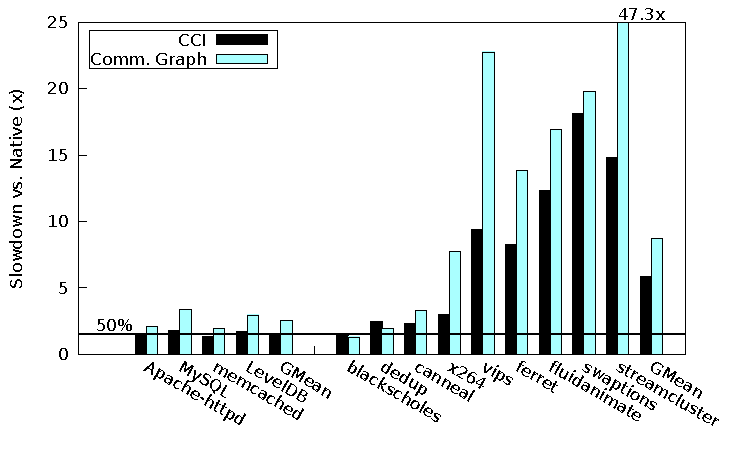
\includegraphics[width=.9\columnwidth]{plots/appperf.pdf}
\caption{\label{fig:perfapps}Performance overheads of CCI-Prev and Graph Collection implemented with \ctraps.}
\end{figure}


\subsection{Characterizing \ctraps}
\label{sec:char}
We characterized the instrumentation pruned by escape analysis.  We report our
results in Table~\ref{tab:char}.  The table shows the percent of
calls pruned and the absolute number of sites in parenthesis.

The data show that escape analysis can prove a substantial fraction of
operations are local and do not require instrumentation.  Across PARSEC,
between 8\% and 30\% of accesses were proved local.  In the server programs, a
larger proportion of accesses were able to be proved local (21\% -- 66\%).  The
difference is likely due to the fact that server threads perform more
independent work (as discussed in Section~\ref{sec:eval:parsecserver}).
Eliminating instrumentation using escape analysis is key to high performance.  

\begin{table}[htb]
\centering
\small
\begin{tabular}{l | r r }
\multirow{3}{*}{\bf Application} & \multicolumn{2}{c}{\bf \em Pruned } \\
               & \multicolumn{2}{c}{\bf \em Static Local}  \\ 
               & \multicolumn{2}{c}{\bf \em Operations}    \\ \hline


Apache         &  21.4\%&(12K)                    \\
MySQL          &  21.3\%&(53K)                    \\
memcached      &  65.8\%&(7.5K)                   \\
LevelDB        &  44.0\%&(4.5K)                   \\ \hline
blackscholes   &   7.5\%&(4)                      \\
dedup          &   22.0\%&(171)                   \\
canneal        &   28.6\%&(226)                   \\
x264           &   29.8\%&(5960)                  \\
vips           &   24.6\%&(9116)                  \\
ferret         &   20.9\%&(792)                   \\
fluidanimate   &   19.6\%&(149)                   \\
streamcluster  &   11.6\%&(47)                    \\
swaptions      &   8.3\% &(19)                    \\
\end{tabular}
\caption{\label{tab:char}Instrumentation pruned by static analysis.}
\end{table}


\section{Related Work}


\paragraph{Debugging with Data Provenance Information}
Prior work has shown that some limited forms of provenance help
with debugging~\cite{badapples, whylineicse, tipslicingsurvey}. 



Bad Value Origin Tracking~\cite{badapples} tracked code that wrote unusable
values into variables~\cite{badapples}. That work showed that revealing the
connection between an unusable value's origin and a failure it causes is
helpful during debugging.  Bad value origin tracking is the closest prior work
to this work~\cite{badapples} and we directly compare to it in our evaluation.
At a high level, bad value origin tracking is like our work because they track
provenance information for debugging, which is a similar goal to ours.  

Bad value origin tracking relates to our work in several other ways.  First,
their technique tracks the provenance of {\em unusable} values only -- a
fraction of all values in an execution.  Our work, instead, tracks provenance
for any value stored in a potentially shared memory location, which includes a
broader set of provenance and targets our technique to concurrency debugging.
Second, for Java programs, bad value origin tracking has runtime overheads
acceptable for production, which was a goal for our system.  Bad value origin
tracking ``piggybacks'' provenance information on storage allocated by the Java
runtime for bad values.  Piggybacking is a key to their low overheads.  For
C/C++, the overhead of bad value origin tracking is much higher.  In C/C++,
they cannot use piggybacking and, instead, use heavy-weight binary
instrumentation with overheads unacceptable for production.  Our technique has
overheads low enough for production for C/C++ programs, especially for server
applications.  Third, their technique does not explicity record thread
information with tracked origins.  Our work focuses on concurrency and we
include thread information.  As we show in Section~\ref{sec:eval:debugging}
thread information is important for some bugs.  

Other work showed that programmers debug more effectively when they can ask
``why'' questions about values during
debugging~\cite{tipslicingsurvey,whylineicse}.  Like our work, the WhyLine
debugger~\cite{whylineicse, whylinechi} allows programmers to ask questions
about why variables hold particular values during debugging.  WhyLine answers
by presenting data- and control-flows that influenced those variables.  WhyLine
differs from our work in that it uses slicing on recorded executions to answer
provenance questions, it has high run time overheads, and does not focus on
concurrency.


\paragraph{Program Slicing}
Program slicing techniques identify useful subsequences of a program's
instructions.   Slicing can work by analyzing program code statically or
analyzing execution traces dynamically.  Many slicing techniques discussed in
the a recent survey~\cite{tipslicingsurvey} monitor control and data
dependences to identify which parts of a program might be relevant to a task
({\em e.g., debugging}).

Thin Slicing~\cite{thinslicing}, is a slicing technique that is related to our
work.  Thin Slicing yields the set of statements that computed on or wrote
values that influenced a ``seed'' variable's value.  Thin
Slicing is similar to our work in that slices provide provenance and it excludes most
control-flow information.  Thin Slicing is different in that it has
overheads too high for production and focused on minimizing the size of each
slice compared to prior slicing techniques. 


\paragraph{Communication and Sharing Analyses in Concurrent Programs}
Several techniques have been proposed analyze dependences and
communication in concurrent programs.  

A closely related recent effort in this space is Octet~\cite{octet} that
captures inter-thread communication soundly and, like \ctraps, can be used to
build dynamic concurrency analyses.  Octet differs from \ctraps in that it is
sound and was built to support analyses on Java programs.  Additionally, Octet
tracks the ``locality state'' of memory locations, rather than the last writer
slice information.  Octet's average run time overhead (26\%) is comparable to
the overhead of both last writer slicing and \ctraps and all three techniques
have low enough overheads in many cases for production use.

CCI~\cite{cci}, Bugaboo~\cite{bugaboo}, LBA~\cite{paralog}, Recon~\cite{recon},
and DefUse~\cite{defuse} all explicitly track some thread interactions.  Unlike
our work, several of these techniques were not designed to run in production
systems~\cite{recon,defuse}.  A distinguishing characteristic of our work is
that it is effective and fast enough for production without the need to
aggregate information from multiple different sampled executions, like
CCI~\cite{cci} does.  Additionally, our system does not require invasive
hardware changes like Bugaboo~\cite{bugaboo} or LBA~\cite{paralog}.

\paragraph{Extensible Program Instrumentation} 
There are many systems for building analyses using program instrumentation.
Binary instrumentation~\cite{pin,dynamorio,valgrind,roadrunner} is general and
tracking provenance and communciation is possible in such systems.  

These systems are similar to \ctraps in that they enable dynamic analyses.
They are different from our work because they rely on dynamic binary
translation, yielding overheads often too high for deployment.  We trade some
generality for performance. \ctraps is effective mainly in the restricted
domain of concurrency analyses, but has overheads low enough for production.
Another difference is that our work handles some of the delicate, performance
sensitive code required concurrency analyses, like last writer tracking.  In
general instrumentation systems, programmers write that code from scratch at
their own risk.  

\section{Conclusions}
In this work we proposed last writer slicing, the first technique to collect data provenance information
that is not limited to certain values, is targeted to concurrent programs, and
has overheads low enough for production use, especially in server programs. 

We developed system support that collects last writer slices with overheads
well within an acceptable range for always-on use in production.  We showed
that during debugging, the provenance information provided by last writer
slices reveals crucial connections between different threads' otherwise
disparate regions of code.  Understanding how code in different threads
interacts is essential to concurrency debugging and this work aids that
understanding.

Using last writer slices, we then built \ctraps, an extensible framework for
implementing concurrent program analyses that interpose on inter-thread
communication.  Trap handlers implement such analyses in just a few lines of
code.  We showed that it is possible to build useful analyses using \ctraps
that are efficient enough for deployment use in an important set of programs
({\em e.g.}, servers, key-value stores, databases, {\em etc.}).  

An interesting direction for future work is to evaluate the role of minimal
hardware support for \ctraps.  We will also further study the impact of
provenance information on debugging in both sequential and concurrent
applications. 




\bibliography{bib}{}
\bibliographystyle{abbrv}

\end{document}
